% PREAMBLE
\documentclass[11pt]{amsart}
\usepackage[T1]{fontenc}
\usepackage{lmodern}
\usepackage{microtype}
\usepackage{amsmath,amssymb}
\usepackage{mathtools}
\usepackage{graphicx}
\usepackage{booktabs}
\usepackage{tikz}
\usepackage[colorlinks=true,linkcolor=blue!45!black,citecolor=blue!45!black,urlcolor=blue!45!black]{hyperref}
\usepackage[capitalize]{cleveref}

\newtheorem{theorem}{Theorem}[section]
\newtheorem{proposition}[theorem]{Proposition}
\newtheorem{lemma}[theorem]{Lemma}
\newtheorem{corollary}[theorem]{Corollary}
\newtheorem{conjecture}[theorem]{Conjecture}
\theoremstyle{definition}
\newtheorem{definition}[theorem]{Definition}
\newtheorem{fact}[theorem]{Fact}
\theoremstyle{remark}
\newtheorem{remark}[theorem]{Remark}

\title{The Dirichlet Inverse of a Digit Design and the Transport of Zeros}
\author{Carlo Mitchener}
\address{MrlyProd, Inc.}
\email{carlo.mitchener@gmail.com}
\date{First published 2026-09-07}

% PAPER
\begin{document}

\begin{abstract}
Cross out some digits of a base and keep the numbers you can still write. That set has a zeta function, a Dirichlet series built from the set alone, and this paper asks what plays the part of the Mobius function for it. The answer is forced: the indicator of the set has a Dirichlet inverse, and it is the Mobius function only when no digit was crossed out. The inverse is worse behaved than the set it inverts. Each zero of the set's zeta function lying to the right of that series' own abscissa of convergence pushes the abscissa of the inverse at least that far right, so the partial sums of the inverse cannot be small. Two such zeros have been located inside certified boxes, one for base three keeping the digits zero and one, one for base ten with the digit nine removed, and in the second case the box lies to the right of the line where the count of all integers sits. The set's own Mobius function therefore does not cancel against the set's own size: it anti-cancels.
\end{abstract}

% TITLE PAGE
\makeatletter
\global\let\titledate\@date
\global\let\paperabstract\@setabstracta
\global\let\@date\@empty
\global\let\@setabstract\relax
\makeatother

\maketitle

\begin{center}
\normalfont\footnotesize\titledate
\end{center}

\vspace*{\stretch{1}}

\begin{center}

\includegraphics[width=0.5\textwidth]{figures/avatar.png}
\end{center}

\vspace*{\stretch{1.25}}

\newpage

\paperabstract

% BODY
\emergencystretch=2em

\section{Introduction}
\label{sec:intro}

Fix a base $q$ and a set $F$ of digits inside $\{0,1,\dots,q-1\}$. The numbers you can still write using only those digits form a set: in base $10$ with the digit $9$ crossed out these are $1,\dots,8,10,\dots,18,20,\dots$, and there are $9^{L}$ of them below $10^{L}$. Call such a set a \emph{design} and write it $S_{F}$. Designs are the standard test bed for analytic number theory on a thin set; Maynard proved that infinitely many of them are prime in base $10$ \cite{may}.

Every set of positive integers has a Dirichlet series, and the design's is
\[
  \zeta_{F}(s) \;=\; \sum_{n \in S_{F}} n^{-s},
\]
which converges exactly in the half-plane $\operatorname{Re} s > \alpha$, where $\alpha = \log_{q} k$ and $k$ is the number of surviving digits. When no digit is crossed out, $S_{F}$ is all of the positive integers, $\alpha = 1$, and $\zeta_{F}$ is Riemann's zeta function.

In that classical case there is a second series, and it is the reason the subject exists. The Mobius function $\mu$ satisfies $\zeta(s) \sum_{n} \mu(n) n^{-s} = 1$: it is exactly the weight you must put on the integers to invert their zeta function. This paper asks the same question of a design. What must you weight $S_{F}$ by to invert $\zeta_{F}$, and how does that weight behave?

\begin{figure}[t]
\centering
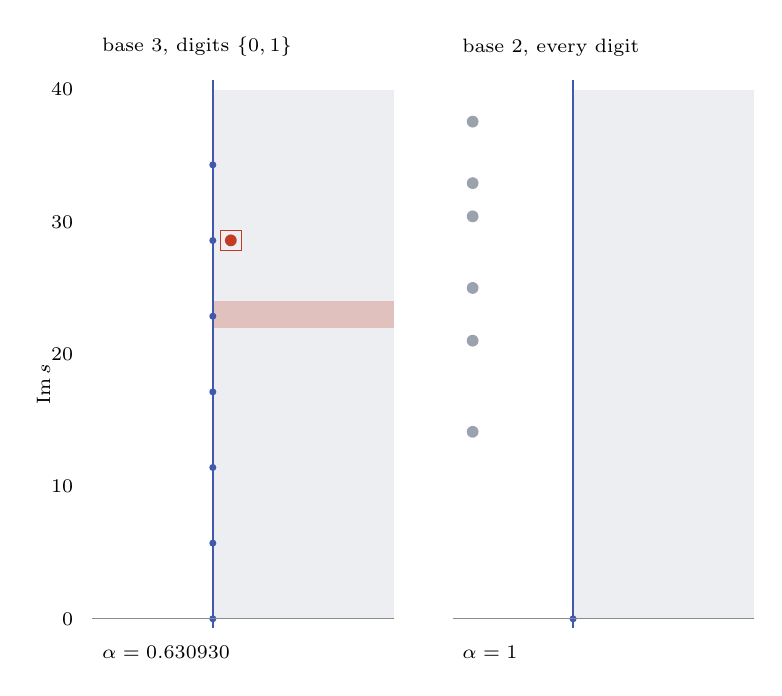
\begin{tikzpicture}[x=1cm,y=1cm]
\definecolor{lane}{HTML}{4059AD}
\definecolor{hit}{HTML}{C23B22}
\definecolor{ctl}{HTML}{9AA3AD}
\definecolor{pale}{HTML}{D5D9E0}
\fill[pale,opacity=0.45] (1.530,0.000) rectangle (3.825,6.720);
\fill[hit,opacity=0.25] (1.530,3.698) rectangle (3.825,4.034);
\draw[lane,thick] (1.530,-0.120) -- (1.530,6.840);
\fill[lane] (1.530,0.000) circle (0.045);
\fill[lane] (1.530,0.961) circle (0.045);
\fill[lane] (1.530,1.922) circle (0.045);
\fill[lane] (1.530,2.882) circle (0.045);
\fill[lane] (1.530,3.843) circle (0.045);
\fill[lane] (1.530,4.804) circle (0.045);
\fill[lane] (1.530,5.765) circle (0.045);
\draw[hit,thin] (1.629,4.676) rectangle (1.889,4.936);
\fill[hit] (1.759,4.806) circle (0.075);
\draw[black!45] (0.000,0.000) -- (3.825,0.000);
\node[anchor=south west,font=\scriptsize] at (0.000,7.020) {base $3$, digits $\{0,1\}$};
\node[anchor=north west,font=\scriptsize] at (0.000,-0.220) {$\alpha = 0.630930$};
\fill[pale,opacity=0.45] (6.105,0.000) rectangle (8.400,6.720);
\draw[lane,thick] (6.105,-0.120) -- (6.105,6.840);
\fill[lane] (6.105,0.000) circle (0.045);
\fill[ctl] (4.830,2.375) circle (0.075);
\fill[ctl] (4.830,3.532) circle (0.075);
\fill[ctl] (4.830,4.202) circle (0.075);
\fill[ctl] (4.830,5.111) circle (0.075);
\fill[ctl] (4.830,5.533) circle (0.075);
\fill[ctl] (4.830,6.314) circle (0.075);
\draw[black!45] (4.575,0.000) -- (8.400,0.000);
\node[anchor=south west,font=\scriptsize] at (4.575,7.020) {base $2$, every digit};
\node[anchor=north west,font=\scriptsize] at (4.575,-0.220) {$\alpha = 1$};
\node[anchor=east,font=\scriptsize] at (-0.120,0.000) {$0$};
\node[anchor=east,font=\scriptsize] at (-0.120,1.680) {$10$};
\node[anchor=east,font=\scriptsize] at (-0.120,3.360) {$20$};
\node[anchor=east,font=\scriptsize] at (-0.120,5.040) {$30$};
\node[anchor=east,font=\scriptsize] at (-0.120,6.720) {$40$};
\node[anchor=east,font=\scriptsize,rotate=90] at (-0.620,3.360) {$\operatorname{Im} s$};
\end{tikzpicture}

\caption{Two Dirichlet series with nonnegative coefficients, each drawn beside its own abscissa of convergence, out to height $40$; the shaded half of each panel is that series' own region of absolute convergence. On the right, the integers: $\zeta$ has abscissa $\operatorname{Re} s = 1$ and, by the Euler product, not one zero in the shaded half. Its six zeros below height $40$ are the grey points, all on $\operatorname{Re} s = 1/2$, all outside the shading. On the left, the design of base $3$ on the digits $\{0,1\}$: its abscissa is $\operatorname{Re} s = \alpha = 0.630930$, the poles of its continuation sit on that line in a lattice of period $2\pi/\log 3$, and two zeros lie inside the shaded half below height $40$, with a third near height $57$. The filled point is the one located inside a certified winding box, at $\rho = 0.720790 + 28.605680\,i$, with the box drawn around it. The strip is the other zero, whose height is censused but whose real part is not pinned, so it is drawn open. Every such zero is transported by \cref{thm:transport} into a lower bound on the design's own M\"obius partial sums.}
\label{fig:zeros}
\end{figure}

The first half of the answer is short and classical in shape. Any arithmetic function $f$ with $f(1) = 1$ has a unique Dirichlet inverse, built by one recursion, and the indicator of $S_{F}$ has $f(1) = 1$ as soon as the digit $1$ survives. So there is a function $\nu_{F}$, and only one, with
\[
  \zeta_{F}(s) N_{F}(s) = 1, \qquad N_{F}(s) = \sum_{n \ge 1} \nu_{F}(n) n^{-s},
\]
and at the full digit set $\nu_{F}$ is $\mu$ on the nose. Nothing here is new; it is the standard construction, recalled in \cref{thm:inverse} to fix notation and to record where $\nu_{F}$ lives. What is worth saying is that $\nu_{F}$ is not $\mu$ cut down to the design, and it is not supported on the design either: it spills onto the multiplicative semigroup that $S_{F}$ generates, and not onto all of that.

The second half is where the design and the integers part company. For the integers, the Euler product $\zeta(s) = \prod_{p} (1 - p^{-s})^{-1}$ forbids a zero anywhere in $\operatorname{Re} s > 1$, and that is why $1/\zeta$ converges as far to the right as $\zeta$ does. A design has no such product. Its indicator is multiplicative only when no digit was crossed out (\cref{thm:wall}), so the Euler route is not narrowed, it is absent, and nothing forbids $\zeta_{F}$ from vanishing inside its own half-plane of absolute convergence. It does vanish there. \cref{fig:zeros} is that statement drawn.

The consequence is one page of elementary complex analysis and is the point of the paper.

\begin{theorem}[The transport, \cref{thm:transport}]
Let $1 \in F$ and let $\rho$ be a zero of $\zeta_{F}$ with $\operatorname{Re}\rho > \alpha$. Then $\sigma_{c}(N_{F}) \ge \operatorname{Re}\rho$, and hence
\[
  \sum_{n \le x} \nu_{F}(n) \;\ne\; O\!\left(x^{\operatorname{Re}\rho - \varepsilon}\right) \quad \text{for every } \varepsilon > 0.
\]
\end{theorem}

The proof is the identity theorem on a connected half-plane and nothing more; it is stated as a theorem because of what it is fed, not because it is deep. What it is fed are two zeros located by the argument principle inside boxes of width $10^{-4}$ (\cref{fact:boxes}). At base $3$ on the digits $\{0,1\}$ the box sits at $\operatorname{Re} s \in [0.72074, 0.72084]$, while the whole design has only $A_{F}(x) \asymp x^{0.630930}$ elements below $x$. So the design's own Mobius function does not cancel against the design's own mass: its partial sums are, along a sequence, larger than the number of terms being summed. At base $10$ with the digit $9$ removed the box sits at $\operatorname{Re} s \in [1.00150, 1.00168]$, to the right of $\operatorname{Re} s = 1$, so the partial sums exceed even the count of all integers below $x$. Both statements are about the limit superior; the finite census is far below both, and \cref{fact:census} says by how much.

This is the observation the paper is for. Everything around it is either classical, elementary, or a measurement, and is labelled as such. In particular the continuation of $\zeta_{F}$ to the whole plane, its pole lattice, and the fact that all of its poles are simple and lie among $\alpha - m + 2\pi i j/\log q$ are Burnol's \cite{bur}; the engine that locates the zeros uses his Proposition 4.1 in a peeled form and claims nothing about it. That $\mu$ is not $q$-automatic, so that no automatic-sequence machinery continues a Mobius-weighted design series, is Coons \cite{coons}. The two other multiplicative structures a design carries, a Lyndon word product and a Beurling system on the primes inside $S_{F}$, are laid out in \cref{sub:products} exactly to say what each one cannot see, and the Beurling comparison is Beurling's \cite{beur} with the cautionary example of Diamond, Montgomery and Vorhauer \cite{dmv}.

Two words on what is not claimed. The transport is one-sided: it bounds $\sigma_{c}(N_{F})$ from below and never from above, so the sentence ``the rightmost zero is the abscissa'' appears nowhere below. And the zero census is resolved rather than certified: the argument principle is run on adaptively refined contours with the largest surviving phase step printed, but nothing here bounds $\zeta_{F}'/\zeta_{F}$ along a contour, so a pair of zeros closer together than the surviving spacing would be invisible to it. The two boxes of \cref{fact:boxes} are the exception and carry a winding number of $1$ each.

\section{The design, its zeta and its inverse}
\label{sec:defs}

Throughout, $q \ge 2$ is an integer base and $F \subseteq \{0,1,\dots,q-1\}$ a set of digits with $k = \#F \ge 1$. Write $e(x) = e^{2\pi i x}$.

\begin{definition}[The design]
\label{def:design}
$S_{F}$ is the set of positive integers every base-$q$ digit of which lies in $F$, and $A_{F}(x) = \#\{n \le x : n \in S_{F}\}$ is its counting function. Write $D_{L}$ for the set of length-$L$ digit strings over $F$ read as base-$q$ integers, so $\# D_{L} = k^{L}$; if $0 \in F$ then $D_{L}$ is the set of elements of $S_{F} \cup \{0\}$ below $q^{L}$ and the $D_{L}$ nest, and if $0 \notin F$ they partition $S_{F}$ by length. The design is \emph{full} when $F = \{0,\dots,q-1\}$, in which case $S_{F}$ is all of $\mathbf{Z}_{>0}$.
\end{definition}

\begin{definition}[The design zeta and the abscissa]
\label{def:zeta}
$\zeta_{F}(s) = \sum_{n \in S_{F}} n^{-s}$ and $\alpha = \log_{q} k$. Since $A_{F}(q^{L}) \le k^{L}$ with equality up to one term, the abscissa of absolute convergence of $\zeta_{F}$ is exactly $\alpha$, and by Landau's theorem on Dirichlet series with nonnegative coefficients $\zeta_{F}$ is singular at $s = \alpha$. Burnol \cite{bur} continues $\zeta_{F}$ meromorphically to $\mathbf{C}$: all poles are simple and lie among the lattice points $s_{m,j} = \alpha - m + 2\pi i j/\log q$ with $m \ge 0$ and $j \in \mathbf{Z}$, the pole at $s_{0,0} = \alpha$ has positive residue, and $\prod_{m \ge 0}(1 - k q^{-s-m}) \zeta_{F}(s)$ is entire. We write $Z(s) = \zeta_{F}(s)(1 - k q^{-s})$ for the \emph{Lyndon cofactor}, which by the same recursion is analytic on $\operatorname{Re} s > \alpha - 1$.
\end{definition}

\begin{definition}[The design Mobius series and the inverse]
\label{def:inverse}
$M_{F}(s) = \sum_{n \in S_{F}} \mu(n) n^{-s}$ is the design Mobius series, the classical $\mu$ read only on the design. It is dominated termwise by $\zeta_{F}$ and so converges absolutely on $\operatorname{Re} s > \alpha$. Separately, when $1 \in F$, $\nu_{F}$ denotes the Dirichlet inverse of the indicator $\mathbf{1}_{S_{F}}$ and $N_{F}(s) = \sum_{n \ge 1} \nu_{F}(n) n^{-s}$ its series, with $\sigma_{c}(N_{F})$ and $\sigma_{a}(N_{F})$ the abscissas of conditional and absolute convergence. These are two different objects and the paper keeps them apart: $M_{F}$ carries the classical arithmetic onto the design, $N_{F}$ is the design's own Mobius function.
\end{definition}

\begin{definition}[The position product]
\label{def:position}
$G_{L}(t) = \prod_{i < L} \sum_{d \in F} e(d q^{i} t)$, a trigonometric polynomial of degree below $q^{L}$, and for an arithmetic function $a$, $A(s,t) = \sum_{n \ge 1} a(n) e(-nt) n^{-s}$.
\end{definition}

\section{Results}
\label{sec:results}

Results are dressed by what stands behind them. A \emph{Theorem} or \emph{Lemma} has a complete proof in \cref{sec:proofs}. A \emph{Fact} is a finite computation, stated with its exact domain and with the script that produced it named; nothing unproved is dressed as a theorem. Every generator named below lives in the public research tree at \url{https://github.com/mrlyprod/mrlyprod} under \texttt{research/lab/}, and \cref{sec:repro} says which of these rows the script shipped with this paper reruns and which it does not.

\subsection{No Euler product over the primes}
\label{sub:wall}

\begin{theorem}[The wall]
\label{thm:wall}
Let $q \ge 2$ and $F \subseteq \{0,\dots,q-1\}$. The indicator $\mathbf{1}_{S_{F}}$ is multiplicative if and only if $F = \{0,\dots,q-1\}$.
\end{theorem}

The proof in \cref{sub:proof-wall} is constructive: for every proper $F$ containing $1$ it writes down a coprime pair witnessing the failure, in three cases. If some digit $c \ge 2$ is missing, take the least such and use the repunits $R_{c}$ and $R_{c+1}$, whose product carries no carry and whose digit set is exactly $\{1,\dots,c\}$. If only the digit $0$ is missing then odd $q$ uses $(2, (q^{2}+1)/2)$ and even $q$ uses $(q^{2}-1, q^{2}+1)$.

\begin{fact}[The wall, swept]
\label{fact:wall}
Over all $8177$ nonempty digit sets with $2 \le q \le 12$: $4083$ have $1 \notin F$ and fail at $f(1) = 1$ alone, $11$ are full, and the constructed witness of \cref{thm:wall} is asserted at each of the remaining $4083$, split $4072$ repunit, $5$ odd base, $6$ even base. An independent minimal search over products up to $4000$ finds a witness for every one of the $4083$; the hardest is $q = 12$, $F = \{1\}$, where the least witness is the pair $(5, 377)$ with product $1885$, against the constructed pair $(13, 157)$. Script of record: \texttt{lab/mrly-euler}, verb \texttt{wall}.
\end{fact}

Consequently no design outside the full digit set carries an Euler product over the primes, and the classical bridge from $\zeta$ to $1/\zeta$ is not narrowed on a design but absent. The pair $\zeta_{F} M_{F}$ measures the damage exactly.

\begin{theorem}[The pair comes apart]
\label{thm:pair}
Let $F$ be strictly inside $\{0,\dots,q-1\}$. Then at least one of the following holds: (i) $1 \notin F$, and the constant coefficient of $\zeta_{F} M_{F}$ is $0$; (ii) some prime $p \in S_{F}$ has $p^{2} \notin S_{F}$, and the coefficient of $\zeta_{F} M_{F}$ at $p^{2}$ is $-1$; (iii) $\zeta_{F} M_{F} = 1$, and then the least element $g > 1$ of $S_{F}$ satisfies $\mu(g) = -1$ and every power $g^{j}$ lies in $S_{F}$. At the full digit set $\zeta_{F} = \zeta$, $M_{F} = 1/\zeta$ and the two are inverse.
\end{theorem}

Clause (iii) is a necessary condition on a hypothetical escapee, not a contradiction, so the theorem is a disjunction and the paper does not upgrade it to a universal. What it says is that an escaping design would have to be squarefree at its smallest nontrivial element and carry that element's whole geometric progression. In practice the pair comes apart at once.

\begin{fact}[Where the pair breaks]
\label{fact:pair}
Over $257$ digit sets ($q \le 8$ with $1 \in F$, plus base $10$ missing $9$, base $10$ missing $0$, and the full sets) the least $n > 1$ at which $\zeta_{F} M_{F}$ has a nonzero coefficient is at most $50$. It is $n = 4$ for base $3$ on $\{0,1\}$, $n = 9$ for base $10$ missing $9$, and $n = 10$ for base $10$ missing $0$ with coefficient $-2$; the eight full sets in the list have no nonzero coefficient below $n = 4000$. Script of record: \texttt{lab/mrly-euler}, verb \texttt{pair}.
\end{fact}

\subsection{The product that survives}
\label{sub:position}

A design does have an exact Euler product. It is not indexed by primes but by digit positions, and it lives in the frequency variable.

\begin{theorem}[The position product]
\label{thm:position}
For every integer $n$,
\[
  \int_{0}^{1} G_{L}(t) e(-nt)\,dt \;=\; \mathbf{1}_{D_{L}}(n),
\]
and hence for every Dirichlet series $\sum_{n \ge 1} a(n) n^{-s}$ absolutely convergent at $s$,
\[
  \sum_{n \in D_{L},\, n \ge 1} a(n) n^{-s} \;=\; \int_{0}^{1} G_{L}(t) A(s,t)\,dt .
\]
\end{theorem}

Taking $a = 1$ makes $A(s,t)$ the periodic zeta function $F(-t,s)$ of DLMF 25.13.1 \cite{dlmf}, and taking $a = \mu$ makes it the Lerch-Mobius series. So $\zeta_{F}$ and $M_{F}$ are two pairings of one set-only product $G_{L}$ against one arithmetic-only kernel: the digit set enters through the positions and never through the primes. Nothing in the proof uses $k = q$, and this is what is left of an Euler product when \cref{thm:wall} has removed the other one.

\begin{remark}[What the position product is for]
\label{rem:whyposition}
Taking $a = \mu$ turns a design Mobius sum into an integral of $G_{L}$ against the Mobius exponential sum $S(x,\theta) = \sum_{n \le x}\mu(n)e(n\theta)$, for which Baker and Harman \cite{bh91} prove $\max_{\theta}|S(x,\theta)| \ll_{\varepsilon} x^{3/4+\varepsilon}$ under the generalized Riemann hypothesis. That is the route by which a bound on $M_{F}$ is usually attempted, and it is not pursued here; \cref{thm:position} is quoted because it is the exact statement of what a design has in place of an Euler product, and because it makes plain that the digit set and the arithmetic occupy separate factors.
\end{remark}

\begin{fact}[The position identity, checked]
\label{fact:position}
The identity of \cref{thm:position} holds to $1.95 \times 10^{-16}$ and $2.04 \times 10^{-16}$ at base $10$ missing $9$ with $L = 3$ and $L = 4$, and to $2.9 \times 10^{-16}$ at base $3$ on $\{0,1\}$ with $L = 3,4,5$, at $s = 3.3$ and $s = 2.7 + 1.9i$, by Gauss-Legendre quadrature on the $q^{L}$ cells. Script of record: \texttt{lab/mrly-euler}, verb \texttt{position}.
\end{fact}

\subsection{The replacement identity}
\label{sub:inverse}

\begin{theorem}[The Dirichlet inverse of a design]
\label{thm:inverse}
Let $1 \in F$. Then $\mathbf{1}_{S_{F}}$ has a unique Dirichlet inverse $\nu_{F}$, given by $\nu_{F}(1) = 1$ and
\[
  \nu_{F}(n) \;=\; -\!\!\sum_{\substack{d \mid n,\; d > 1 \\ d \in S_{F}}}\!\! \nu_{F}(n/d) \qquad (n > 1),
\]
so that $\zeta_{F}(s) N_{F}(s) = 1$ as formal Dirichlet series and pointwise wherever both converge absolutely. The support of $\nu_{F}$ lies inside the multiplicative semigroup generated by $S_{F}$, and strictly inside it. At the full digit set $\nu_{F} = \mu$.
\end{theorem}

The existence and uniqueness of a Dirichlet inverse for any $f$ with $f(1) \ne 0$ is entirely classical and the one-line induction is recalled in \cref{sub:proof-inverse} only to fix the recursion the script runs. What the statement adds is the location of the support. At base $3$ on $\{0,1\}$ the integers $9$, $27$ and $36$ lie in the semigroup generated by $S_{F}$ and have $\nu_{F} = 0$, while $16 = 4 \cdot 4$, $48 = 4 \cdot 12$ and $52 = 4 \cdot 13$ lie in that semigroup and outside $S_{F}$. So four sets are in play and no two of them coincide: the design $S_{F}$; the semigroup it generates; the Beurling integers built on the primes lying in $S_{F}$, treated in \cref{sub:products}; and the support of $\nu_{F}$.

\begin{fact}[The inverse, computed]
\label{fact:inverse}
On the full digit set $\nu_{F} = \mu$ term for term to $n = 131072$ at $q = 2$ and to $n = 177147$ at $q = 3$. Off it, the partial sums of $N_{F}(\sigma)$ meet $1/\zeta_{F}(\sigma)$ to $1.60 \times 10^{-3}$ at $\sigma = 0.8008$ and to $1.96 \times 10^{-4}$ at $\sigma = 0.9208$ at base $3$ on $\{0,1\}$, and to $1.72 \times 10^{-2}$ at $\sigma = 1.0816$ and $2.39 \times 10^{-3}$ at $\sigma = 1.2016$ at base $10$ missing $9$. All four abscissas sit above the $\operatorname{Re}\rho$ of \cref{fact:boxes} and nothing is evaluated below it. Script of record: \texttt{lab/mrly-pairing}, verb \texttt{inverse}.
\end{fact}

\subsection{The transport}
\label{sub:transport}

\begin{theorem}[The transport]
\label{thm:transport}
Let $1 \in F$ and suppose $\zeta_{F}$ has a zero $\rho$ with $\operatorname{Re}\rho > \alpha$. Then
\[
  \sigma_{c}(N_{F}) \;\ge\; \operatorname{Re}\rho,
\]
and consequently $\sum_{n \le x} \nu_{F}(n) \ne O(x^{\operatorname{Re}\rho - \varepsilon})$ for every $\varepsilon > 0$.
\end{theorem}

\begin{remark}[What the transport is and is not]
\label{rem:onesided}
The proof is the identity theorem applied on the connected half-plane $\operatorname{Re} s > \max(\sigma_{c}(N_{F}), \alpha)$, which is free of the pole lattice, plus the standard implication from a partial-sum bound to an abscissa. It is elementary, and it is stated as a theorem for what it is fed rather than for its depth. It is also strictly one-sided: it bounds $\sigma_{c}(N_{F})$ from below with no error term and no hypothesis beyond $1 \in F$, and the converse inequality $\sigma_{c}(N_{F}) \le \sup \operatorname{Re}\rho$ is not proved here or anywhere the author knows. In particular ``the rightmost zero is the abscissa'' is not a statement of this paper.
\end{remark}

\subsection{Zeros to the right of the abscissa}
\label{sub:zeros}

For a Dirichlet series with nonnegative coefficients, having a zero inside the half-plane of absolute convergence is possible in general: $1 + 2^{-s}$ has abscissa $-\infty$ and zeros at $(2m+1)\pi i/\log 2$. The content here is not the principle but the object. A design zeta is an infinite series with a genuine finite abscissa, and it has zeros to the right of it, which the Euler product forbids for $\zeta$.

\begin{fact}[The zero census]
\label{fact:count}
The census counts zeros of the Lyndon cofactor $Z(s) = \zeta_{F}(s)(1 - k q^{-s})$, which is analytic on $\operatorname{Re} s > \alpha - 1$, on the single strip $\alpha - 0.92 < \operatorname{Re} s < \alpha + 3.02$, $0.02 < \operatorname{Im} s < 60$, split at $\operatorname{Re} s = \alpha$ exactly, so nothing is left unscanned against the pole line. Base $3$ on $\{0,1\}$ carries $3$ zeros to the right of the abscissa and $20$ to the left; base $10$ missing $9$ carries $13$ right and $25$ left; base $3$ on $\{0,2\}$ carries $3$ right, in the same three boxes as $\{0,1\}$. The base $2$ full digit set is the control and each side names its object: zeros of $\zeta$ in $\alpha + 0.02 < \operatorname{Re} s < \alpha + 3.02$ count $0$, computed and not quoted; zeros of $\zeta$ in $\alpha - 0.98 < \operatorname{Re} s < \alpha - 0.02$ count $13$, the first thirteen below $\operatorname{Im} s = 60$; and the teeth of $1 - 2 q^{-s}$, which lie exactly on $\operatorname{Re} s = \alpha$ and are not zeros of $\zeta$, bring the one-strip cofactor count to $19 = 13 + 6$ with $6 = \lfloor 60 \log 2 / 2\pi \rfloor$. To the right of the abscissa no continuation is used: the positive series converges absolutely there and the ladder only rearranges it. The largest surviving phase step on any census contour is $0.9896$ and the largest propagated error bound met at any census evaluation is $9.99 \times 10^{-11}$, both printed beside every count. The count is resolved and not certified: nothing here bounds $\zeta_{F}'/\zeta_{F}$ on the contour, so a zero pair closer than the surviving spacing would stay invisible. Script of record: \texttt{lab/design-zeta}.
\end{fact}

\begin{fact}[Two certified boxes]
\label{fact:boxes}
The argument principle returns winding number $1$ on the rectangle $\operatorname{Re} s \in [0.72074, 0.72084]$, $\operatorname{Im} s \in [28.60563, 28.60573]$ at base $3$ on $\{0,1\}$, with contour minimum $|\zeta_{F}| = 8.298 \times 10^{-4}$ against a propagated evaluation bound of $6.284 \times 10^{-30}$; and winding number $1$ on $\operatorname{Re} s \in [1.00150, 1.00168]$, $\operatorname{Im} s \in [2.73915, 2.73925]$ at base $10$ missing $9$, with contour minimum $6.865 \times 10^{-4}$ against $2.798 \times 10^{-23}$. The control rectangle $\operatorname{Re} s \in [0.99900, 1.00050]$, $\operatorname{Im} s \in [2.73810, 2.74030]$ at base $10$ returns winding $0$. Each box therefore contains exactly one zero, and five digits of $\operatorname{Re}\rho$ are certified in each case. Both boxes lie strictly to the right of the respective abscissa, $\alpha = 0.6309297536$ and $\alpha = 0.9542425094$. Script of record: \texttt{lab/mrly-pairing}, verb \texttt{box}, on the engine of \texttt{lab/design-zeta}.
\end{fact}

\begin{corollary}[Anti-cancellation]
\label{cor:anti}
At base $3$ on $\{0,1\}$, $\sum_{n \le x} \nu_{F}(n) \ne O(x^{0.72074 - \varepsilon})$ for every $\varepsilon > 0$, while $A_{F}(x) \asymp x^{0.6309297}$. At base $10$ missing $9$, $\sum_{n \le x} \nu_{F}(n) \ne O(x^{1.00150 - \varepsilon})$ for every $\varepsilon > 0$, and the exponent exceeds $1$.
\end{corollary}

So on these two designs the limit superior of the design's own Mertens function is strictly larger than the design's own mass, and at base $10$ missing $9$ it is larger than the count of all integers below $x$. A conjecture of the form ``the design's Mobius partial sums are $O(x^{\alpha/2 + \varepsilon})$'' is therefore false for $\nu_{F}$ on these two designs and can only be carried by $\mu$ restricted to $S_{F}$, that is by $M_{F}$; and \cref{thm:pair} is exactly what keeps the zeros of $\zeta_{F}$ from reaching $M_{F}$.

\begin{fact}[The census is far below the limit superior]
\label{fact:census}
The two statements of \cref{cor:anti} are about a limit superior and the finite census does not see them. Pointwise the running maximum of $\sum_{n \le x} \nu_{F}(n)$ reaches only $0.0738$ of $A_{F}(x)$ at base $3$ on $\{0,1\}$ at level $L = 16$, and $0.0847$ of $x$ at base $10$ missing $9$ at $L = 7$. Its growth per level at base $10$ missing $9$ reads $9.4474$, $11.5000$, $10.2220$, $10.0354$ at $L = 4,\dots,7$, against $q^{\operatorname{Re}\rho} = 10.036661$ and the trivial rate $k = 9$; only the last of the four lands on the predicted rate, so quoting it alone would be selection. The ratio of running maximum to $A_{F}(q^{L})$ rises $0.1043$, $0.1094$, $0.1398$, $0.1588$, $0.1771$ at $L = 3,\dots,7$. At base $3$ on $\{0,1\}$ the geometric mean of the four steps $L = 12,\dots,16$ is $2.059$ against $q^{\operatorname{Re}\rho} = 2.207512$ and the trivial $k = 2$, while the arithmetic mean of the five printed level ratios is $1.9972$, below the trivial rate: at this depth the census cannot separate the two rates. Script of record: \texttt{lab/mrly-pairing}, verb \texttt{inverse}.
\end{fact}

\subsection{The glue that gains nothing}
\label{sub:glue}

Since $\zeta_{F} M_{F} \ne 1$, write $\zeta_{F} M_{F} = 1 + D_{F}$ and ask whether $D_{F}$ is cheap enough that $M_{F} = (1 + D_{F})/\zeta_{F}$ buys anything. It is not.

\begin{proposition}[The abscissa of the defect]
\label{prop:glue}
Let $0, 1 \in F$ and $k < q$. Then $\sigma_{a}(D_{F}) \le \alpha$. Moreover, if $\sigma_{c}(D_{F}) < \alpha$ then $M_{F}(\sigma) \to 0$ as $\sigma \to \alpha^{+}$ along the real axis.
\end{proposition}

The second half is Landau: $\zeta_{F}$ has nonnegative coefficients and abscissa $\alpha$, so it is singular there and $\zeta_{F}(\sigma) \to +\infty$, while $D_{F}$ would be holomorphic at $\alpha$. There is no circularity, since $M_{F}$ is dominated termwise by $\zeta_{F}$ and so converges absolutely at every $\sigma > \alpha$ with no hypothesis at all.

\begin{fact}[The defect is not cheap]
\label{fact:glue}
Write $P(x) = \sum_{n \le x} c_{F}(n)$ for the partial sums of the coefficients of $\zeta_{F} M_{F}$. If $\sigma_{c}(D_{F})$ were below $\alpha$ then $P(x) = o(x^{\alpha})$ would follow. Sampled at four phases per level, because $P(x)/x^{\alpha}$ is log-periodic and sampling only at $x = q^{L}$ aliases every Fourier mode onto one number, $P(x)/x^{\alpha}$ reads $0.493767$, $0.699235$, $0.758519$, $0.587055$ at base $3$ on $\{0,1\}$ out to $x = 3^{17.75}$, bounded away from $0$ and from infinity. So $\sigma_{c}(D_{F}) = \alpha$ there. At base $10$ missing $9$ the same four phases read $-0.011742$, $0.033309$, $0.058519$, $0.073298$ out to $x = 10^{6.75}$, which is a smaller and less settled reading and is not claimed as a determination. Script of record: \texttt{lab/mrly-pairing}, verb \texttt{glue}.
\end{fact}

\begin{corollary}[The glue is lossy]
\label{cor:lossy}
On a design where \cref{thm:transport} applies, $M_{F} = (1 + D_{F}) N_{F}$ with $\sigma_{c}(N_{F}) > \alpha$, so factoring $M_{F}$ through the design's own Mobius function replaces the trivial exponent $\alpha$ by something strictly worse. The route is not neutral, it is lossy.
\end{corollary}

\subsection{Two other products, and what each one sees}
\label{sub:products}

Two more multiplicative structures sit near a design, and each is worth stating precisely, because each is blind to something.

\begin{theorem}[The Lyndon word product]
\label{thm:lyndon}
Give the free monoid on the alphabet $F$ the norm $N(w) = q^{|w|}$. Then
\[
  \sum_{w} N(w)^{-s} \;=\; \frac{1}{1 - k q^{-s}} \;=\; \prod_{L \ge 1} \left(1 - q^{-Ls}\right)^{-c_{k}(L)},
\]
where $c_{k}(L) = \frac{1}{L}\sum_{d \mid L}\mu(d)k^{L/d}$ is the number of Lyndon words of length $L$ over a $k$-letter alphabet. This is an exact Euler product whose primes are the Lyndon words. This zeta has no zero, its own Mobius function is supported on the empty word and the single letters so its Mertens function is $1 - k$ at every norm above $1$, and its poles are exactly the design pole lattice $s = \alpha + 2\pi i m/\log q$.
\end{theorem}

The reading is that the design's multiplicative shadow carries the pole lattice and no Riemann-hypothesis content whatever, and that all such content of $\zeta_{F}$ sits in the cofactor $Z(s) = \zeta_{F}(s)(1 - k q^{-s})$, which is precisely the function \cref{fact:count} censuses.

\begin{fact}[The Lyndon expansion]
\label{fact:lyndon}
The product of \cref{thm:lyndon} expands to $1/(1 - ku)$ through $u^{16}$ at $k = 2,3,4,9,10$, and $c_{2}(L)$ for $L = 1,\dots,10$ is $2, 1, 2, 3, 6, 9, 18, 30, 56, 99$, the sequence A001037 \cite{a1037}. Script of record: \texttt{lab/mrly-euler}, verb \texttt{word}.
\end{fact}

\begin{theorem}[The Beurling system collapses at a non-unit digit gcd]
\label{thm:beurling}
Let $N_{F}^{B}$ be the free abelian monoid on the primes lying in $S_{F}$, so that $\mu$ restricts to it and the Beurling zeta is $\prod_{p \in S_{F}}(1 - p^{-s})^{-1}$. If $\gcd(F) = a > 1$ then every element of $S_{F}$ is a multiple of $a$; when $a$ is prime the only prime of the design is $a$, $N_{F}^{B}$ is the powers of $a$ and the Beurling Mertens function $M_{B}(x)$ vanishes for $x \ge a$; when $a$ is composite $S_{F}$ contains no prime at all, $N_{F}^{B} = \{1\}$ and $M_{B} \equiv 1$.
\end{theorem}

So the Beurling route is blind to every scaled column, base $10$ on $\{0,4,8\}$ for instance, while the scaling theorem of \cref{sub:scaling} reads those columns exactly. And $N_{F}^{B}$ is not $S_{F}$: the two sets are different and the census below is a census on the wrong one, deliberately, as the control it is.

\begin{fact}[The Beurling census to $10^{6}$]
\label{fact:beurling}
Base $3$ on $\{0,2\}$ has the single prime $2$ and $M_{B} \equiv 0$ past $2$. Base $3$ on $\{0,1\}$ has $525$ primes, $N_{F}^{B}(920483) = 2198$, running maximum $|M_{B}| = 98$ and exponent $\log(\max)/\log x = 0.3339$ against $\alpha/2 = 0.3155$. Base $10$ missing $9$ has $35139$ primes, $N_{F}^{B}(10^{6}) = 488864$ against $x^{\alpha} = 531441$, $M_{B}(10^{6}) = 1860$ with running maximum $1866$, and exponent $0.4203$, $0.4882$, $0.5452$ at $x = 10^{4}, 10^{5}, 10^{6}$ against $\alpha/2 = 0.4771$, where the full base $10$ control reads $0.4084$, $0.4241$, $0.4276$ at the same points against its own $\alpha/2 = 0.5$ and reproduces $M(10^{4}) = -23$, $M(10^{5}) = -48$, $M(10^{6}) = 212$, A084237 \cite{a084237}. What this reads is a level and not a trend: $+0.068$ over $\alpha/2$ for the design against $-0.072$ for the control, with a running maximum climbing in both. There is cancellation, $0.545$ against the trivial $\alpha = 0.954$, and it sits above $\alpha/2$. Script of record: \texttt{lab/mrly-euler}, verb \texttt{beurling}.
\end{fact}

A Beurling system need not satisfy a Riemann hypothesis at all. Beurling introduced generalised prime systems in \cite{beur}, and Diamond, Montgomery and Vorhauer \cite{dmv} construct one whose integer counting function is $\kappa x + O(x^{\theta})$ with $1/2 < \theta < 1$ and whose zeta still has infinitely many zeros on $\sigma = 1 - a/\log t$. So no regularity of the counting function of a design forces anything about $M_{B}$, and \cref{fact:beurling} is offered as a measurement and not as evidence for a conjecture.

\subsection{Scaled digit sets share a zero set}
\label{sub:scaling}

\begin{theorem}[Scaling]
\label{thm:scaling}
Let $a$ be a positive integer with $a \max F \le q - 1$, so that $aF \subseteq \{0,\dots,q-1\}$. Then $m \mapsto am$ is a carry-free bijection $S_{F} \to S_{aF}$ and
\[
  \zeta_{aF}(s) \;=\; a^{-s}\,\zeta_{F}(s).
\]
The factor $a^{-s}$ has no zero and no pole, so $\zeta_{aF}$ and $\zeta_{F}$ have exactly the same zeros, and residues in the ratio $a^{-s_{m,j}}$. The proof uses $0 \in F$ nowhere.
\end{theorem}

\begin{fact}[Scaling, checked]
\label{fact:scaling}
Base $3$ on $\{0,2\}$ against base $3$ on $\{0,1\}$: the identity of \cref{thm:scaling} holds to $5.6 \times 10^{-43}$ at three points, and on the censused strip $\alpha < \operatorname{Re} s < \alpha + 3.02$, $0.02 < \operatorname{Im} s < 60$ the two censuses coincide box for box, winding $1$ in $\operatorname{Im} s \in [22.01, 24.01]$, in $[28.01, 30.01]$ and in $[56.00, 58.00]$ for both and winding $0$ in every other box. To the left of the abscissa $\{0,2\}$ is not censused and is inferred from the theorem. Script of record: \texttt{lab/design-zeta}.
\end{fact}

\subsection{Open problems}
\label{sub:open}

The transport is one-sided and the paper leaves it there. Nothing above bounds $\sigma_{c}(N_{F})$ from above, so it is not known whether the abscissa of the design's own Mobius series equals the supremum of the real parts of the zeros of $\zeta_{F}$, or even whether that supremum is finite. Nothing above determines the locus of those zeros: the three at base $3$ on $\{0,1\}$ below height $60$ are located and counted, and no law is offered for where the next one sits, nor for how their number grows with height. Two of the four designs the generators carry, base $4$ and base $5$ on $\{0,1\}$, have no zero census at all, so \cref{cor:anti} is silent on them and it is not known whether every proper design has a zero to the right of its abscissa or only some do. The zero counts of \cref{fact:count} are resolved and not certified, and certifying them needs a bound on $\zeta_{F}'/\zeta_{F}$ along a contour that no one here has. The determination $\sigma_{c}(D_{F}) = \alpha$ of \cref{fact:glue} rests on a measurement at one design and wants a proof. And the conjecture the whole apparatus was built to test, that $\sum_{n \le x, n \in S_{F}} \mu(n)$ is $O(x^{\alpha/2 + \varepsilon})$, is untouched by everything above: \cref{cor:anti} rules out $\nu_{F}$ as its carrier and says nothing whatever about $\mu$ restricted to $S_{F}$.

\section{Proofs}
\label{sec:proofs}

\subsection{The wall}
\label{sub:proof-wall}

\begin{proof}[Proof of \cref{thm:wall}]
Sufficiency is immediate: on the full digit set $\mathbf{1}_{S_{F}}$ is identically $1$ on the positive integers, which is completely multiplicative.

For necessity, let $F$ be proper. A multiplicative $f$ has $f(1) = 1$, so $1 \in F$ is forced, and if $1 \notin F$ we are done. Assume $1 \in F$. The missing digits are nonempty, and either some missing digit is at least $2$, or the only missing digit is $0$.

\emph{Case A: some $c \in \{2,\dots,q-1\}$ is missing.} Take the least such $c$, so $\{1,\dots,c-1\} \subseteq F$ and $c \notin F$. Write $R_{a} = (q^{a}-1)/(q-1)$ for the repunit with $a$ ones. Its digits are all $1$, so $R_{c}, R_{c+1} \in S_{F}$, and $\gcd(R_{a},R_{b}) = R_{\gcd(a,b)}$ gives $\gcd(R_{c},R_{c+1}) = R_{1} = 1$. Now
\[
  R_{c} R_{c+1} \;=\; \sum_{i < c} \sum_{j < c+1} q^{i+j},
\]
and the number of pairs $(i,j)$ with $0 \le i \le c-1$, $0 \le j \le c$ and $i + j = m$ is $\min(m+1,\, c,\, 2c-m)$, which is at most $c \le q - 1$. No carry occurs, so that count is literally the $q^{m}$ digit of the product, and as $m$ runs over $0,\dots,2c-1$ the digits run over exactly $\{1,\dots,c\}$. Since $c \notin F$ the product leaves $S_{F}$, while both factors lie in it, so $f(R_{c}R_{c+1}) = 0 \ne 1 = f(R_{c})f(R_{c+1})$.

\emph{Case B: only $0$ is missing, so $F = \{1,\dots,q-1\}$.} If $q$ is odd then $q \ge 3$ and $(q^{2}+1)/2 = \frac{q-1}{2}\,q + \frac{q+1}{2}$, whose two digits $\frac{q-1}{2}$ and $\frac{q+1}{2}$ both lie in $\{1,\dots,q-1\}$; moreover $q^{2} \equiv 1 \pmod 8$, so $(q^{2}+1)/2$ is odd and is coprime to $2$. Both $2$ and $(q^{2}+1)/2$ lie in $S_{F}$, while the product $q^{2}+1$ has base-$q$ digits $1,0,1$ and does not. If $q$ is even then $q^{2}-1$ and $q^{2}+1$ are both odd and differ by $2$, hence coprime; the product $q^{4}-1$ has every digit equal to $q-1$ and so lies in $S_{F}$, while $q^{2}+1$ has the digit $0$ and does not, so here $f(mn) = 1 \ne 0 = f(m)f(n)$. This case covers $q = 2$, $F = \{1\}$, with the pair $(3,5)$ and product $15 = 1111_{2}$.
\end{proof}

\begin{proof}[Proof of \cref{thm:pair}]
Write $c_{F}(n) = \sum_{de = n,\ d,e \in S_{F}} \mu(e)$ for the $n$-th coefficient of $\zeta_{F}M_{F}$. If $1 \notin F$ then $n = 1$ has no admissible factorisation and $c_{F}(1) = 0$, which is (i). If some prime $p \in S_{F}$ has $p^{2} \notin S_{F}$, the divisors of $p^{2}$ are $1, p, p^{2}$, and the only factorisation with both sides in $S_{F}$ is $(p,p)$, so $c_{F}(p^{2}) = \mu(p) = -1$, which is (ii).

Suppose neither holds and $c_{F}(n) = 0$ for every $n > 1$. Let $g$ be the least element of $S_{F}$ greater than $1$, so that no divisor of anything lying strictly between $1$ and $g$ is in $S_{F}$. Taking $n = g$, the admissible factorisations are $(1,g)$ and $(g,1)$, so $0 = c_{F}(g) = \mu(g) + 1$ and $\mu(g) = -1$; in particular $g$ is squarefree. Now induct: suppose $g^{i} \in S_{F}$ for all $i < j$, which holds vacuously at $j = 1$. In $c_{F}(g^{j})$ write the factorisation as $d \cdot e$ with $e \in S_{F}$ and $\mu(e) \ne 0$, so $e$ is a squarefree divisor of $g^{j}$, hence a divisor of $g$. If $e = 1$ then $d = g^{j}$ must lie in $S_{F}$ and the term is $\mu(1) = 1$. If $e > 1$ then $e \in S_{F}$ forces $e \ge g$ and $e \mid g$ forces $e = g$, so $d = g^{j-1}$, which lies in $S_{F}$ by the induction hypothesis, and the term is $\mu(g) = -1$. Hence $0 = c_{F}(g^{j}) = \mathbf{1}[g^{j} \in S_{F}] - 1$, so $g^{j} \in S_{F}$. That is (iii). At the full digit set $\zeta_{F} = \zeta$ and $M_{F} = 1/\zeta$, so the two are inverse.
\end{proof}

\subsection{The position product}
\label{sub:proof-position}

\begin{proof}[Proof of \cref{thm:position}]
Expanding the product over positions,
\[
  G_{L}(t) \;=\; \sum_{(d_{0},\dots,d_{L-1}) \in F^{L}} e\!\left(\Big(\sum_{i<L} d_{i} q^{i}\Big) t\right),
\]
\begin{sloppypar}
so $\int_{0}^{1} G_{L}(t)e(-nt)\,dt$ counts the strings in $F^{L}$ with $\sum_{i<L} d_{i}q^{i} = n$. Since $F \subseteq \{0,\dots,q-1\}$, that is the number of base-$q$ representations of $n$ with $L$ digits, all in $F$, which is $1$ if $n \in D_{L}$ and $0$ otherwise, by uniqueness of the expansion. For the second identity, $|G_{L}| \le k^{L}$ is bounded and $\sum_{n} |a(n)| n^{-\operatorname{Re} s}$ converges, so the sum defining $A(s,t)$ converges uniformly in $t$ and may be integrated term by term against $G_{L}$; the first identity then selects exactly the $n \in D_{L}$.
\end{sloppypar}
\end{proof}

\subsection{The Dirichlet inverse and the transport}
\label{sub:proof-inverse}

\begin{proof}[Proof of \cref{thm:inverse}]
Since $1 \in F$ we have $\mathbf{1}_{S_{F}}(1) = 1$, and the classical construction applies: define $\nu_{F}(1) = 1$ and, for $n > 1$, let $\nu_{F}(n)$ be given by the stated recursion, which is exactly the requirement $\sum_{d \mid n,\ d \in S_{F}} \nu_{F}(n/d) = 0$ solved for the $d = 1$ term. Uniqueness is the same recursion read forwards. The identity $\zeta_{F}N_{F} = 1$ is the resulting convolution $\mathbf{1}_{S_{F}} * \nu_{F} = \delta$ read as Dirichlet series, valid formally and, where both series converge absolutely, pointwise.

For the support, induct on $n$: $\nu_{F}(n)$ is a sum of terms $\nu_{F}(n/d)$ with $d \in S_{F}$, $d > 1$, so if $\nu_{F}(n) \ne 0$ then $\nu_{F}(n/d) \ne 0$ for some such $d$, and by induction $n/d$ lies in the multiplicative semigroup generated by $S_{F}$; hence so does $n$. That the containment is strict is witnessed at base $3$ on $\{0,1\}$ by $9 = 3 \cdot 3$, $27$ and $36$, which lie in the semigroup and have $\nu_{F} = 0$. On the full digit set the recursion is $\nu_{F}(n) = -\sum_{d \mid n, d > 1} \nu_{F}(n/d)$, which is the defining recursion of $\mu$, so $\nu_{F} = \mu$.
\end{proof}

\begin{proof}[Proof of \cref{thm:transport}]
Write $\sigma_{0} = \sigma_{c}(N_{F})$ and suppose, for contradiction, that $\sigma_{0} < \operatorname{Re}\rho$. Put
\[
  U \;=\; \{s : \operatorname{Re} s > \max(\sigma_{0}, \alpha)\},
\]
a connected half-plane. On $U$ the series $N_{F}$ converges and defines a holomorphic function, and $\zeta_{F}$ is holomorphic there as well, since its abscissa of absolute convergence is $\alpha$ and every pole of its continuation has real part at most $\alpha$. On the sub-half-plane where both series converge absolutely, the convolution identity $\mathbf{1}_{S_{F}} * \nu_{F} = \delta$ gives $\zeta_{F}(s)N_{F}(s) = 1$. Both sides are holomorphic on the connected open set $U$, so by the identity theorem $\zeta_{F}N_{F} = 1$ throughout $U$, and in particular $\zeta_{F}$ has no zero in $U$. But $\operatorname{Re}\rho > \alpha$ and $\operatorname{Re}\rho > \sigma_{0}$ place $\rho \in U$, a contradiction. Hence $\sigma_{0} \ge \operatorname{Re}\rho$.

For the last clause, if $\sum_{n \le x}\nu_{F}(n) = O(x^{\theta})$ then the standard partial-summation estimate gives $\sigma_{c}(N_{F}) \le \theta$. Taking $\theta = \operatorname{Re}\rho - \varepsilon$ would contradict the bound just proved.
\end{proof}

\begin{proof}[Proof of \cref{prop:glue}]
The $n$-th coefficient of $\zeta_{F}M_{F}$ is $c_{F}(n) = \sum_{de=n,\ d,e \in S_{F}}\mu(e)$, so $|c_{F}(n)|$ is at most the $n$-th coefficient of $\zeta_{F}^{2}$, a Dirichlet series with nonnegative coefficients and abscissa of absolute convergence $\alpha$. Hence $\sigma_{a}(D_{F}) \le \alpha$.

For the second half, $\zeta_{F}$ has nonnegative coefficients and abscissa $\alpha$, so by Landau's theorem it is singular at $s = \alpha$ and $\zeta_{F}(\sigma) \to +\infty$ monotonically as $\sigma \to \alpha^{+}$ along the real axis. If $\sigma_{c}(D_{F}) < \alpha$ then $D_{F}$ is holomorphic at $\alpha$ and in particular bounded near it, so
\[
  M_{F}(\sigma) \;=\; \frac{1 + D_{F}(\sigma)}{\zeta_{F}(\sigma)} \;\longrightarrow\; 0 .
\]
There is no circularity: $M_{F}$ is dominated termwise by $\zeta_{F}$, hence converges absolutely at every $\sigma > \alpha$ with no hypothesis on the size of $\sum_{n \le x, n \in S_{F}} \mu(n)$.
\end{proof}

\subsection{The two other products, and scaling}
\label{sub:proof-products}

\begin{proof}[Proof of \cref{thm:lyndon}]
The free monoid on $F$ has $k^{L}$ words of length $L$, each of norm $q^{L}$, so with $u = q^{-s}$ the norm zeta is $\sum_{L \ge 0} k^{L} u^{L} = 1/(1-ku)$ for $\operatorname{Re} s > \alpha$. By the Chen-Fox-Lyndon theorem every word over $F$ factors uniquely as a non-increasing product of Lyndon words, so the free monoid is equinumerous by norm with the free abelian monoid on the Lyndon words; counting the latter by norm gives
\[
  \frac{1}{1-ku} \;=\; \prod_{L \ge 1}\left(1-u^{L}\right)^{-c_{k}(L)},
\]
with $c_{k}(L)$ the number of Lyndon words of length $L$ over a $k$-letter alphabet, which is $\frac{1}{L}\sum_{d \mid L}\mu(d)k^{L/d}$ by the standard necklace count. This is an Euler product with the Lyndon words as primes. It has no zero, since $1/(1-ku)$ never vanishes. Its own Mobius function is the coefficient sequence of $1 - ku$, that is $1$ at the empty word and $-1$ at each of the $k$ letters and $0$ beyond, so its summatory function is $1 - k$ at every norm above $1$. Its poles are the solutions of $kq^{-s} = 1$, that is $s = \log_{q}k + 2\pi i m/\log q = \alpha + 2\pi i m /\log q$, which is the design pole lattice of \cref{def:zeta}.

Since the free monoid is not the free abelian monoid on Lyndon words but only equinumerous with it by norm, this is a statement about norms and carries no arithmetic beyond them; and since $Z(s) = \zeta_{F}(s)(1-kq^{-s})$ divides out exactly this factor, whatever zero structure $\zeta_{F}$ has beyond the lattice sits in $Z$.
\end{proof}

\begin{proof}[Proof of \cref{thm:beurling}]
If $\gcd(F) = a > 1$ then every base-$q$ digit of every $n \in S_{F}$ is divisible by $a$, hence so is $n$. If $a$ is prime, an element of $S_{F}$ that is prime must therefore equal $a$, and $a \in S_{F}$ exactly when $a$ is a one-digit element, which it is; so the primes of the design are $\{a\}$, $N_{F}^{B}$ is $\{a^{j} : j \ge 0\}$, and its Mobius sum telescopes to $\mu(1) + \mu(a) = 0$ at every $x \ge a$. If $a$ is composite, no element of $S_{F}$ is prime at all, $N_{F}^{B} = \{1\}$ and $M_{B} \equiv 1$.
\end{proof}

\begin{proof}[Proof of \cref{thm:scaling}]
Let $m \in S_{F}$ have base-$q$ digits $d_{i} \in F$. Since $a d_{i} \le a \max F \le q-1$, the integer $am = \sum_{i} (a d_{i}) q^{i}$ is presented with digits $ad_{i}$, all lying in $aF$ and all below $q$, so this is its base-$q$ expansion and $am \in S_{aF}$. Conversely, if $n \in S_{aF}$ has digits $e_{i} \in aF$, then each $e_{i} = a d_{i}$ with $d_{i} \in F$, and $m = \sum_{i} d_{i}q^{i}$ lies in $S_{F}$ with $am = n$. So $m \mapsto am$ is a bijection $S_{F} \to S_{aF}$ and
\[
  \zeta_{aF}(s) \;=\; \sum_{m \in S_{F}} (am)^{-s} \;=\; a^{-s}\zeta_{F}(s)
\]
on $\operatorname{Re} s > \alpha$, hence on the whole plane by continuation. The factor $a^{-s}$ is entire and never zero, so $\zeta_{aF}$ and $\zeta_{F}$ have the same zeros with the same multiplicities, and residues in the ratio $a^{-s_{m,j}}$. Nothing in the argument used $0 \in F$.
\end{proof}

\section{Reproducibility}
\label{sec:repro}

Two scripts accompany this paper. Both are plain \texttt{python3} with no dependency beyond the standard library, take no arguments, write nothing outside \texttt{figures/}, and are run from the lane root. Every assertion names the value obtained and the value wanted, and a failure stops the script.

\texttt{python3 scripts/verify.py} runs in about one second in a few tens of megabytes and covers the following, in order.
\begin{itemize}
\item \emph{The wall}, \cref{thm:wall}: all $246$ nonempty digit sets of the bases $2 \le q \le 7$. Of these $120$ have $1 \notin F$ and $6$ are full; at each of the remaining $120$ the constructed pair is built, asserted coprime, and asserted to break multiplicativity in one direction or the other. The branch split is $114$ repunit, $3$ odd base, $3$ even base, and the pairs at base $3$ on $\{0,1\}$, base $2$ on $\{1\}$ and base $12$ on $\{1\}$ are checked individually. This is a smaller domain than \cref{fact:wall}, which the script does not rerun.
\item \emph{The inverse}, \cref{thm:inverse}: $\nu_{F}$ at base $3$ on $\{0,1\}$ computed to $n = 3^{8} = 6561$ from the recursion, then the convolution $\mathbf{1}_{S_{F}} * \nu_{F}$ recomputed by an independent loop over $a \in S_{F}$ and asserted equal to $\delta$ at every $n \le 6561$, so that $\zeta_{F}N_{F} = 1$ is checked as a coefficient identity by a second code path. The semigroup generated by $S_{F}$ is built to the same bound: $9$, $27$ and $36$ are asserted inside it with $\nu_{F} = 0$, and $16$, $48$ and $52$ inside it and outside $S_{F}$; and $\nu_{F}(n) \ne 0$ is asserted to imply membership at every $n \le 6561$. The control is the full digit set, where $\nu_{F} = \mu$ is asserted term for term to $n = 8192$ at $q = 2$ and $n = 6561$ at $q = 3$, against an independent sieve for $\mu$.
\item \emph{The position product}, \cref{thm:position}: the identity in its exact grid form. Since $G_{L}$ is a trigonometric polynomial of degree below $q^{L}$, the integral equals the $q^{L}$-point Riemann sum exactly, so the check is an identity between finite sums and not a quadrature. Base $3$ on $\{0,1\}$ at $L = 5$ for every $n < 243$, worst error $1.4 \times 10^{-15}$; base $10$ missing $9$ at $L = 3$ for every $n < 1000$, worst error $4.4 \times 10^{-15}$.
\item \emph{The Lyndon product}, \cref{thm:lyndon}: the expansion of $\prod_{L}(1-u^{L})^{-c_{k}(L)}$ through $u^{16}$ in exact integer arithmetic, asserted equal to $\sum_{i}k^{i}u^{i}$ at $k = 2, 3, 4, 9, 10$, and $c_{2}(L)$ asserted against the first ten terms of A001037.
\item \emph{The design zeta and the two box centres}: the peel recursion of \cref{def:zeta}, namely $(1-kq^{-s})\zeta_{F}(s) = \sum_{a \in F, a \ne 0}a^{-s} + \sum_{l \ge 1}\binom{-s}{l}q^{-s-l}\gamma_{l}\zeta_{F}(s+l)$ with $\gamma_{l} = \sum_{a \in F}a^{l}$, which is Burnol's Proposition 4.1 \cite{bur}, solved bottom-up over $260$ integer shifts in double precision, the highest shifts evaluated by direct summation. It is validated at $s = 2$ against the direct sum over the elements of $S_{F}$ below $q^{L}$, inside the proved truncation tail $k(kq^{-s})^{L}/(1-kq^{-s})$: the discrepancy is $1.392\times10^{-10}$ against a tail of $4.1\times10^{-10}$ at base $3$ on $\{0,1\}$ with $L = 15$, and $6.042\times10^{-6}$ against $5.8\times10^{-5}$ at base $10$ missing $9$ with $L = 5$. It is then re-evaluated at the two box centres of \cref{fact:boxes}, returning $|\zeta_{F}| = 7.46\times10^{-5}$ at base $3$ and $1.22\times10^{-5}$ at base $10$, against $9.78\times10^{-1}$ and $6.87\times10^{-1}$ one unit higher in $\operatorname{Im} s$.
\item \emph{Scaling}, \cref{thm:scaling}: $S_{2F} = 2S_{F}$ as sets below $3^{9}$ at base $3$, and $\zeta_{\{0,2\}}(s) = 2^{-s}\zeta_{\{0,1\}}(s)$ to $1.4\times10^{-16}$ at $s = 0.6+3.1i$ through the same evaluator.
\end{itemize}

One caution about the last item, and it is the important one. The smallness of $|\zeta_{F}|$ at the two box centres is an \emph{illustration and not a certificate}. It is exactly what a box five digits wide and a derivative of size $O(1)$ predict, and a small value of a function bounds nothing about its zeros without a lower bound on the derivative, which is taken nowhere here. What certifies each zero is the winding number of \cref{fact:boxes}, computed by the argument principle in \texttt{lab/mrly-pairing}, verb \texttt{box}, on the interval-bounded engine of \texttt{lab/design-zeta}. Note also that a raw truncation of the Dirichlet series cannot serve even as an illustration: to the right of the abscissa the tail after $L$ digit levels is of size $(kq^{-\operatorname{Re}\rho})^{L}$, which is $0.906^{L}$ at base $3$ on $\{0,1\}$ and $0.897^{L}$ at base $10$ missing $9$, so no reachable depth makes it small. The peel recursion is a resummation of the same series and is what makes the evaluation possible at all.

\begin{sloppypar}
The script does not rerun the ten Facts of \cref{sec:results}, namely \cref{fact:wall,fact:pair,fact:position,fact:inverse}, \cref{fact:count,fact:boxes,fact:census}, and \cref{fact:glue,fact:beurling,fact:scaling}. Those come from three generators of the public research tree at \url{https://github.com/mrlyprod/mrlyprod}, under \texttt{research/lab/}:
\end{sloppypar}
\begin{itemize}
\item \texttt{mrly-euler}, verbs \texttt{wall}, \texttt{pair}, \texttt{position}, \texttt{word}, \texttt{beurling};
\item \texttt{mrly-pairing}, verbs \texttt{inverse}, \texttt{glue}, \texttt{box};
\item \texttt{design-zeta}, the census and the evaluation engine.
\end{itemize}
Of these, \texttt{position} runs in a few minutes and every other \texttt{mrly-euler} verb in seconds; \texttt{glue} and \texttt{inverse} take about thirty seconds each and \texttt{box} about twenty; the full census of \texttt{design-zeta} to $\operatorname{Im} s = 60$ is the longest run in the group. Their exact finite domains are the ones stated in each Fact above and repeated in each generator's own documentation.

\texttt{python3 scripts/figure.py} runs in under a second. It writes \texttt{figures/figure.svg}, the picture the repository README embeds, and \texttt{figures/zeros.tex}, the Ti\emph{k}Z version of \cref{fig:zeros} that this document includes; both are drawn from the same data, namely the exact pole lattice $\alpha + 2\pi i j/\log q$, the certified box of \cref{fact:boxes}, the two uncertified height bands of \cref{fact:count}, and the first six ordinates of $\zeta$ on the control column. \texttt{tectonic paper.tex} rebuilds \texttt{paper.pdf}.

\section*{Acknowledgments}

This paper was developed and verified in collaboration with Claude (Anthropic). The author takes sole responsibility for every claim.

\begin{thebibliography}{9}

\bibitem{a1037}
OEIS Foundation Inc., \emph{Entry A001037: number of binary Lyndon words of length $n$}, The On-Line Encyclopedia of Integer Sequences. \url{https://oeis.org/A001037}

\bibitem{a084237}
OEIS Foundation Inc., \emph{Entry A084237: Mertens's function $M(10^{n})$}, The On-Line Encyclopedia of Integer Sequences. \url{https://oeis.org/A084237}

\bibitem{bh91}
R. C. Baker and G. Harman, \emph{Exponential sums formed with the M\"obius function}, J. London Math. Soc. (2) \textbf{43} (1991), no. 2, 193--198. \href{https://doi.org/10.1112/jlms/s2-43.2.193}{doi:10.1112/jlms/s2-43.2.193}

\bibitem{beur}
A. Beurling, \emph{Analyse de la loi asymptotique de la distribution des nombres premiers g\'en\'eralis\'es. I}, Acta Math. \textbf{68} (1937), 255--291. \href{https://doi.org/10.1007/BF02546666}{doi:10.1007/BF02546666}

\bibitem{bur}
J.-F. Burnol, \emph{On the analytic continuation of Dirichlet series with missing digits}, preprint, 2026. \href{https://arxiv.org/abs/2602.19727}{arXiv:2602.19727}

\bibitem{coons}
M. Coons, \emph{(Non)automaticity of number theoretic functions}, J. Th\'eor. Nombres Bordeaux \textbf{22} (2010), no. 2, 339--352. \href{https://doi.org/10.5802/jtnb.718}{doi:10.5802/jtnb.718}

\bibitem{dmv}
H. G. Diamond, H. L. Montgomery and U. M. A. Vorhauer, \emph{Beurling primes with large oscillation}, Math. Ann. \textbf{334} (2006), no. 1, 1--36. \href{https://doi.org/10.1007/s00208-005-0638-2}{doi:10.1007/s00208-005-0638-2}

\bibitem{dlmf}
NIST Digital Library of Mathematical Functions, \emph{\S25.13, Periodic Zeta Function}. \url{https://dlmf.nist.gov/25.13}

\bibitem{may}
J. Maynard, \emph{Primes with restricted digits}, Invent. Math. \textbf{217} (2019), 127--218. \href{https://doi.org/10.1007/s00222-019-00865-6}{doi:10.1007/s00222-019-00865-6}

\end{thebibliography}

\end{document}
